\documentclass{article}
\usepackage{xcolor}
\usepackage{titleps}
\usepackage[letterpaper, margin=0.95in]{geometry}
\usepackage{url}
\usepackage{amsmath}
\usepackage{amssymb}
\usepackage{wrapfig}
\usepackage{float}
\usepackage{mathtools}
\usepackage{enumitem}
\usepackage{tabu}
\usepackage{parskip}
\usepackage{natbib}
\usepackage{listings}
\usepackage[utf8]{inputenc} % allow utf-8 input
\usepackage[T1]{fontenc}    % use 8-bit T1 fonts
\usepackage[hidelinks]{hyperref}       % hyperlinks
\usepackage{wrapfig}
\usepackage{url}            % simple URL typesetting
\usepackage{booktabs}       % professional-quality tables
\usepackage{amsfonts}       % blackboard math symbols
\usepackage{nicefrac}       % compact symbols for 1/2, etc.
\usepackage[expansion=false]{microtype}      % microtypography
\usepackage{xcolor}         % colors
\usepackage{amsmath,amssymb} % define this before the line numbering.
\usepackage{makecell}
% % Support for easy cross-referencing
\usepackage{graphics} % for pdf, bitmapped graphics files
\usepackage{colortbl}
\usepackage{xcolor}
% \usepackage{epsfig} % for postscript graphics files
\usepackage{empheq}
%\usepackage{mathptmx} % assumes new font selection scheme installed
% \usepackage{times} % assumes new font selection scheme installed
\usepackage{bm}
\usepackage{bbding} 
% \usepackage{cite}
\usepackage{diagbox}
\usepackage[linesnumbered,ruled]{algorithm2e}
% \usepackage{ulem} %to strike the words
% \usepackage{hyperref}
% \usepackage{soul}

\newcommand{\cmark}{\ding{51}}%
\newcommand{\xmark}{\ding{55}}%
% \definecolor{themeblue}{RGB}{57, 162, 219}
% \definecolor{themegreen}{RGB}{87, 204, 153}
% \definecolor{forestgreen}{RGB}{47, 159, 87}

\usepackage[capitalize]{cleveref}
% \usepackage{todonotes}
\usepackage{float}
\usepackage{booktabs}
\usepackage{multirow}
%\usepackage{ bbold }
\usepackage{mathrsfs}
\usepackage[utf8]{inputenc}
%\usepackage{subfigure}
\usepackage{pifont}
\usepackage{threeparttable}

\usepackage{hyperref}
\usepackage[color=red]{todonotes}
\usepackage{forest}
\definecolor{light-yellow}{HTML}{FFE5CC}
\newcounter{RNum}
\renewcommand{\theRNum}{\arabic{RNum}}
\newcommand{\Remark}{\noindent\textbf{Remark}~\refstepcounter{RNum}\textbf{\theRNum}: }
\newcommand{\fref}[1]{Fig.~\ref{#1}}
\newcommand{\sref}[1]{Section~\ref{#1}}
\newcommand{\tref}[1]{Table~\ref{#1}}
\newcommand{\appref}[1]{Appendix~\ref{#1}}
\newcommand{\highlight}[1]{\noindent\quad\textbf{#1}:~}
\newcommand{\myparagraph}[1]{\noindent\textbf{#1}~}

\newpagestyle{ruled}
{\sethead{CMU 16-831}{Intro to Robot Learning}{Fall 2025}\headrule
  \setfoot{}{}{}}
\pagestyle{ruled}

\renewcommand\makeheadrule{\color{black}\rule[-.75\baselineskip]{\linewidth}{0.4pt}}
\renewcommand*\footnoterule{}

\begin{document}
\lstset{basicstyle = \ttfamily,columns=fullflexible,
backgroundcolor = \color{light-yellow}
}

\begin{centering}
    {\Large Assignment 1: Imitation Learning} \\
    \vspace{.25cm}
    \textbf{Andrew ID:} \texttt{lzaceria} \\
    \textbf{Collaborators:} \texttt{YOUR COLLABORATORS}\\ 
\end{centering}

\vspace{.5cm}

\section{Behavioral Cloning (9.75 pt)}
\subsection{Part 2 (1.5 pt)}
\# TODO
\begin{table}[!h]
  \centering
  \caption{Report your result in this table.}
    \begin{tabular}{cccccc}
    \toprule[1.0pt]
    Metric/Env & Ant-v2 & Humanoid-v2 & Walker2d-v2 & Hopper-v2 & HalfCheetah-v2 \\
    \midrule
    Mean  & 4713.653 & 10344.518 & 5566.846 & 3772.670 & 4205.778 \\
    Std.  & 12.197 & 20.981 & 9.238  & 1.948  & 83.039 \\
    \bottomrule[1.0pt]
    \end{tabular}%
  \label{tab:p2}%
\end{table}%

\subsection{Part 3 (5.25 pt)}
\# TODO
\begin{table}[htbp]
  \centering
  \caption{BC vs Expert performance comparison. \\ Hyperparameters: learning\_rate=4e-3, n\_layers=5, n\_iter=1, eval\_batch\_size=5000, ep\_len=1000 (approximately 5 evaluation trajectories per environment). \\ Ant-v2 achieves 91.7\% expert performance (>30\% threshold), while Humanoid-v2 achieves 3.1\% expert performance (<30\% threshold).}
    \begin{tabular}{ccccc}
    \toprule[1.0pt]
    Env   & \multicolumn{2}{c}{Ant-v2} & \multicolumn{2}{c}{Humanoid-v2} \\
    \midrule
    Metric & Mean  & Std.  & Mean  & Std. \\
    Expert & 4713.653 & 12.197 & 10344.518 & 20.981 \\
    BC    & 4323.741 & 509.877 & 320.130 & 48.081 \\
    \bottomrule[1.0pt]
    \end{tabular}%
  \label{tab:p3}%
\end{table}%

\subsection{Part 4 (3 pt)}
I tested the learning rate hyperparameter on Ant-v2, varying it from 1e-4 to 5e-2. Learning rate controls the gradient step size during training.

The results show optimal performance at lr=4e-3 (4103 return), with our Part 3 result of 4324 falling within the standard deviation range. Lower rates (1e-4) lead to undertraining, while higher rates (5e-2) cause instability. The performance drops significantly at the extremes.

See Figure~\ref{fig:1} on the next page for a summary of these results.

\begin{figure}[H]
	\centering
	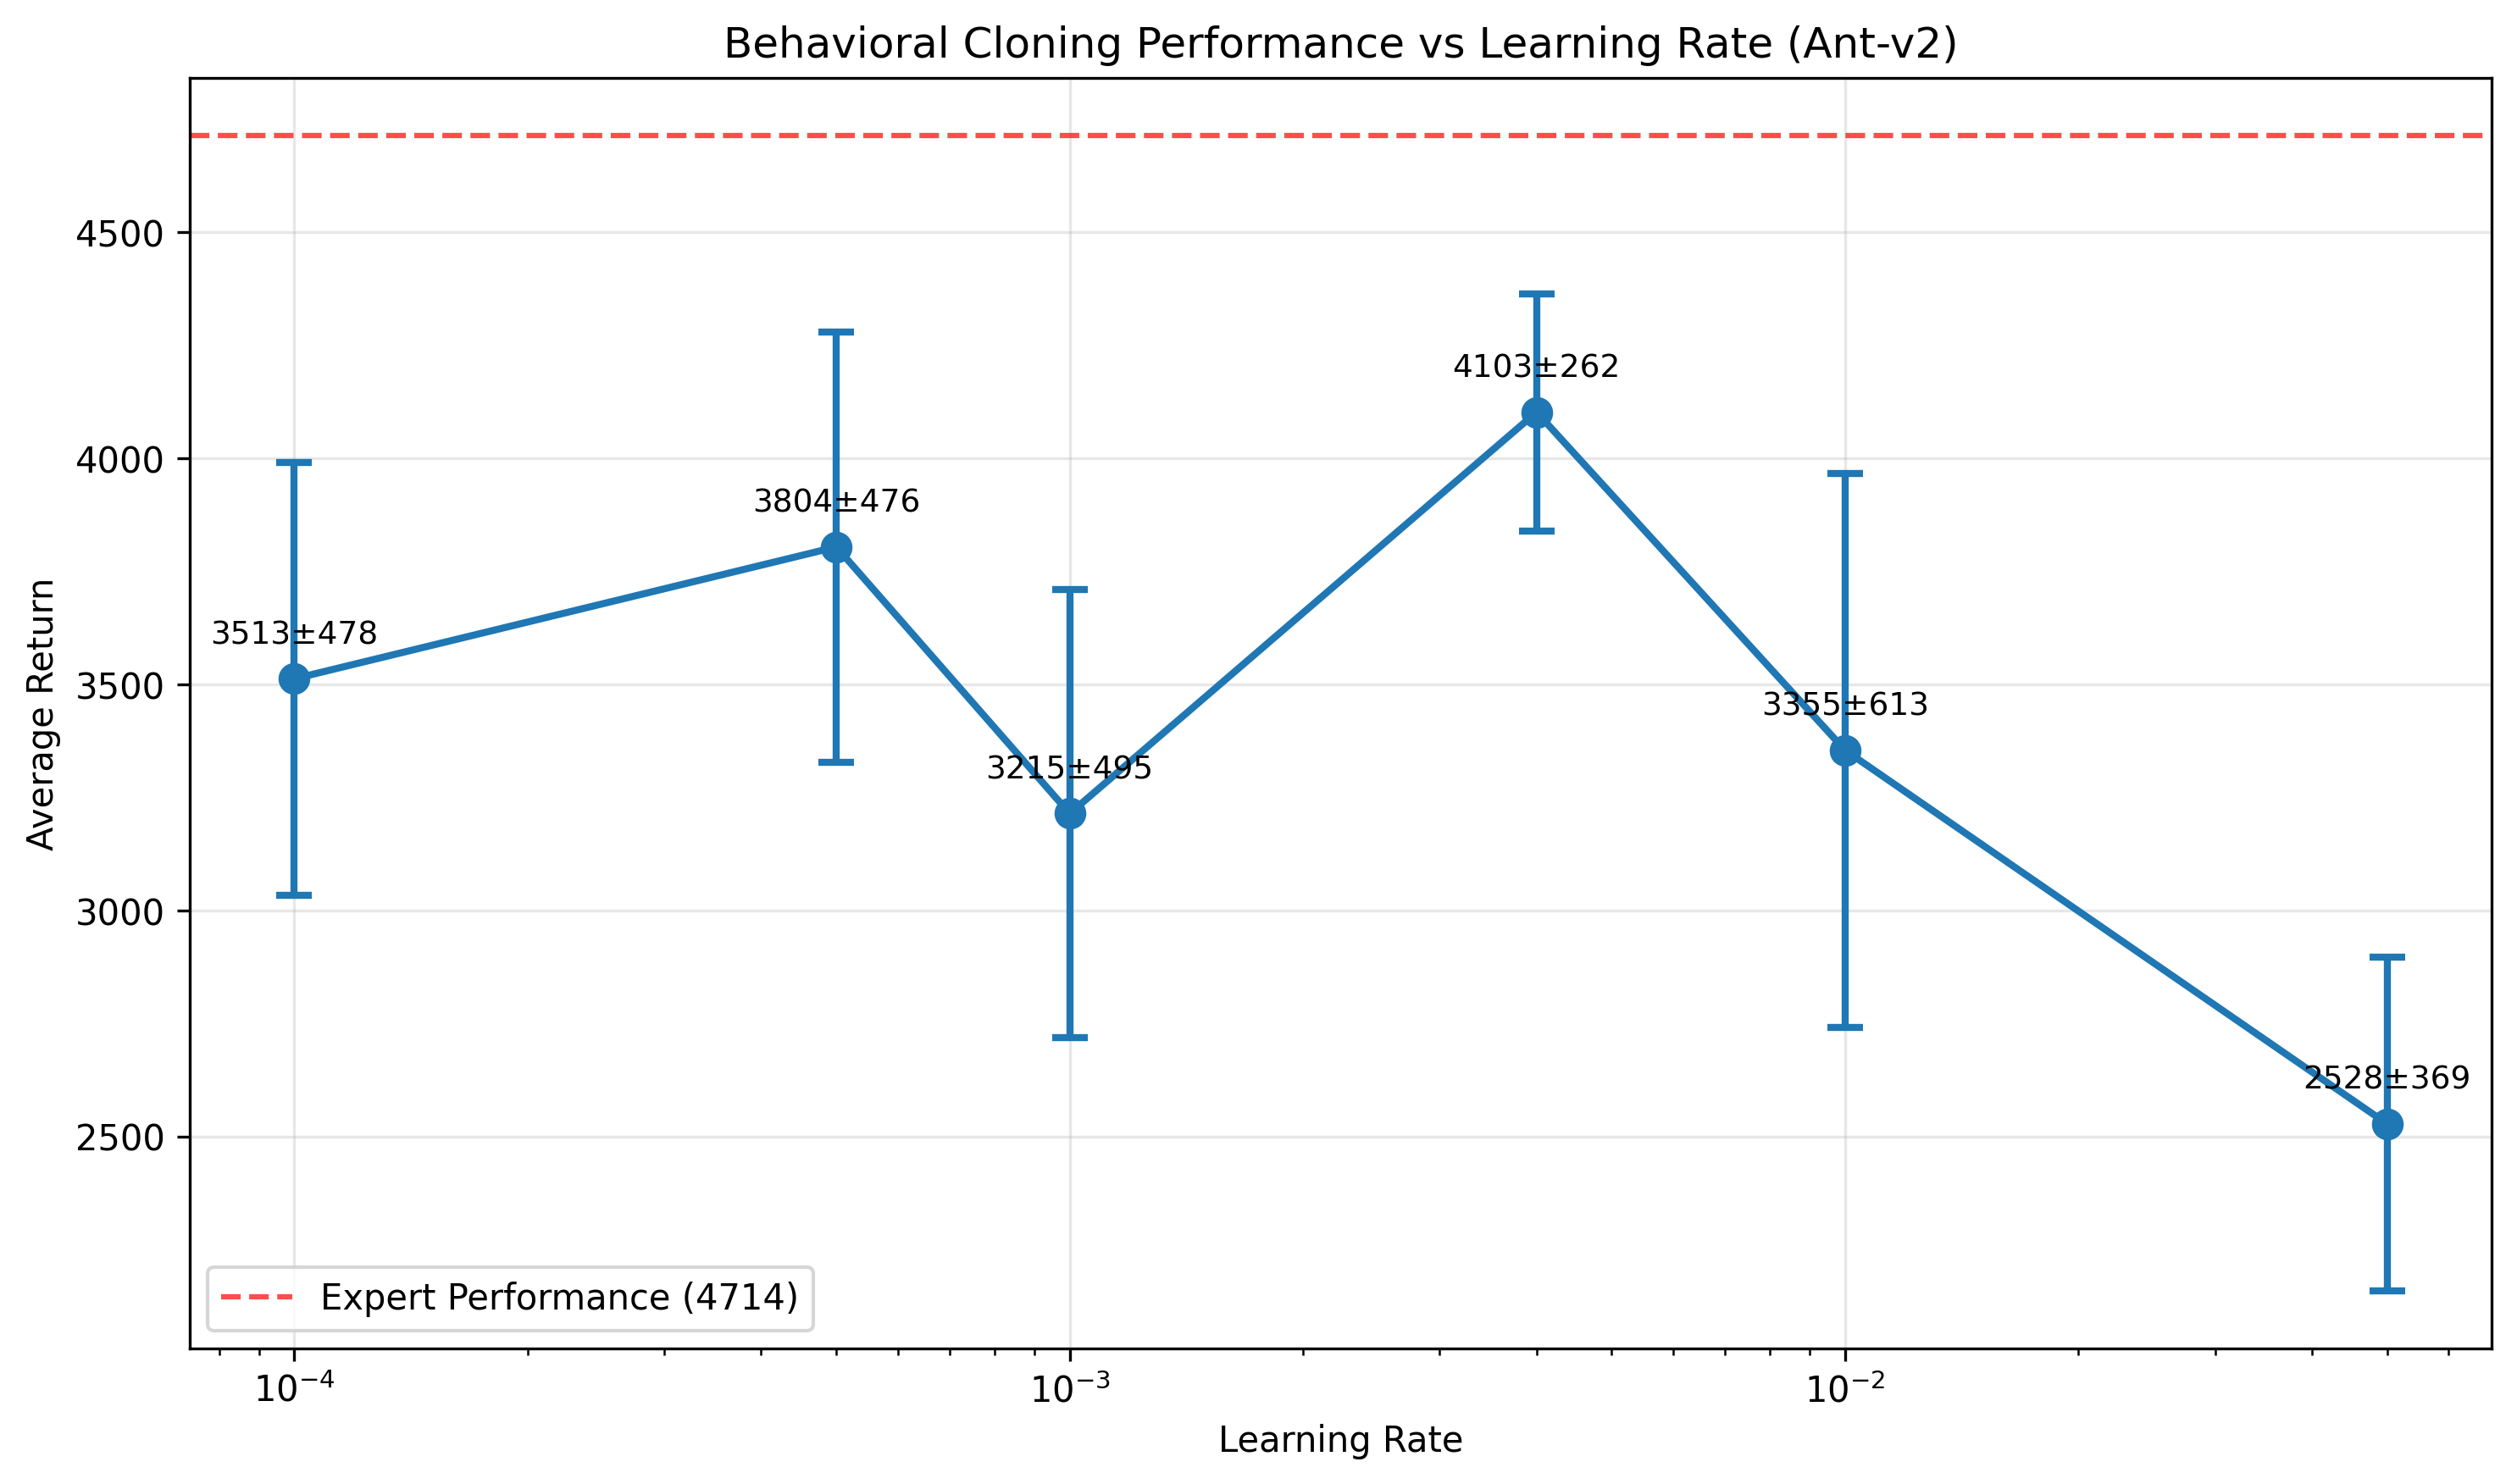
\includegraphics[width=0.8\columnwidth]{learning_rate_experiment_ant.png}
	\caption{BC agent's performance varies with the learning rate parameter in the Ant-v2 environment. Peak performance at lr=4e-3, with worse performance at very low and high rates. Error bars show std over 5 runs.}
	\label{fig:1}
\end{figure}

\vspace{2cm} % Add vertical space to help the figure appear above the next section

\section{DAgger (5.25 pt)}
\subsection{Part 2 (5.25 pt)}
Report the results for Ant-v2 and HalfCheetah-v2 in \fref{fig:p5}:
\begin{figure*}[!h]
	\centering
	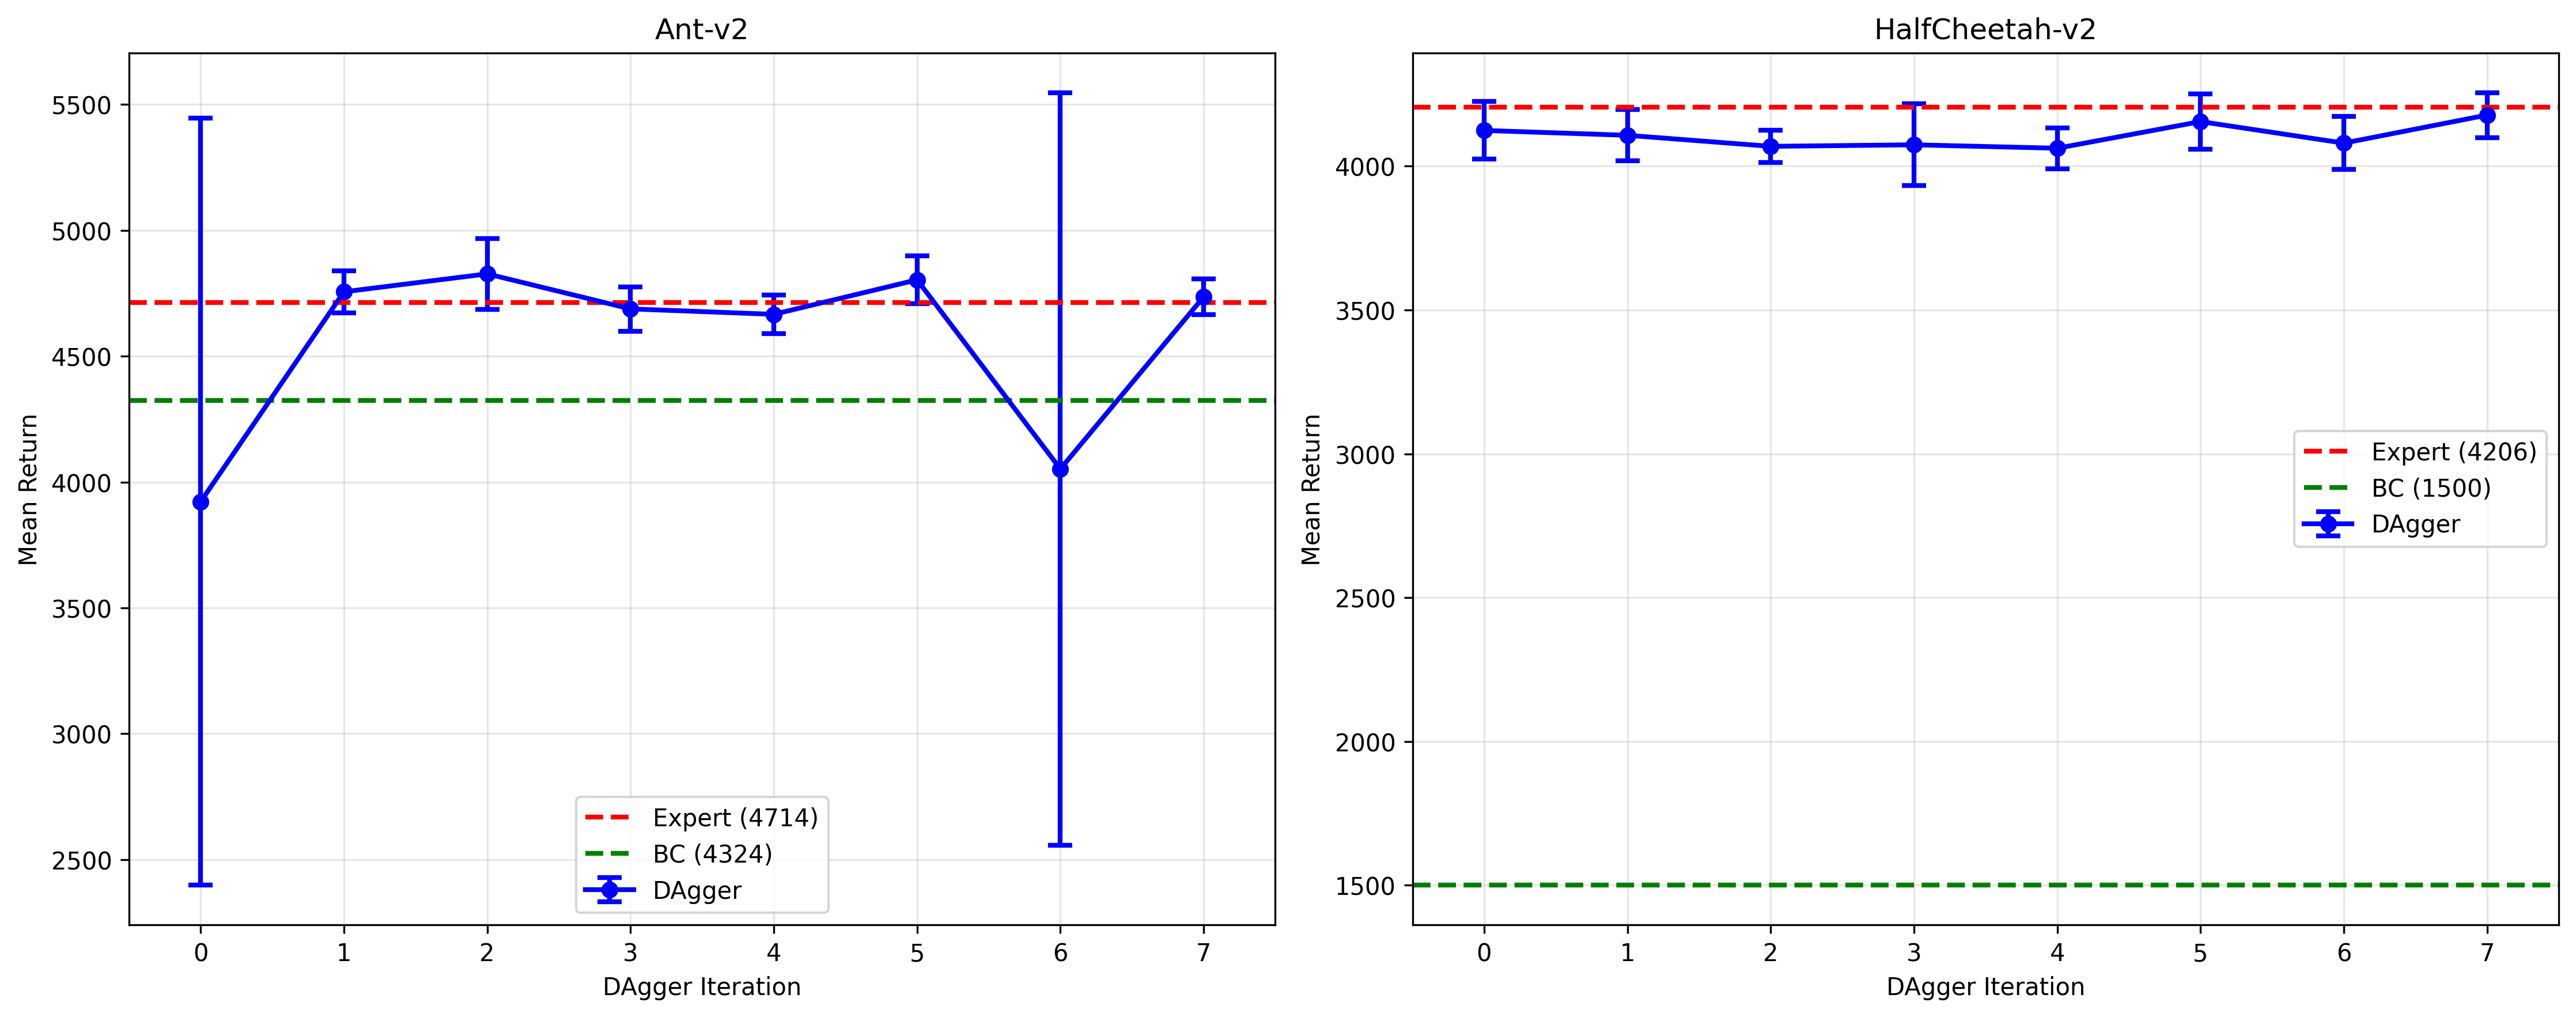
\includegraphics[width=0.8\textwidth]{dagger_results_figure.png}
	\caption{Learning curve, plotting the number of DAgger iterations vs. the policy's mean return, with error bars to show the standard deviation. Please show the Ant-v2 environment results on the left and the results from HalfCheetah-v2 on the right. Network architecture: 3-layer MLP. DAgger was run for 8 iterations with expert relabeling at each iteration.}
	\label{fig:p5}
\end{figure*}

\end{document}
